\documentclass[12pt, a4paper]{report}
\usepackage{graphicx}
\usepackage[export]{adjustbox}
\usepackage{amsmath}
\graphicspath{{images/}}
\title{Centrality Measures}
\date{MONSOON SEMESTER 2023}
\begin{document}
\maketitle

Centrality measures are a vital tool for understanding networks. These algorithms use graph theory to calculate the importance of any given node in a network. Centrality has different types and each type or metric defines the \emph{“importance”} of a node from different perspectives and further provides relevant analytical information about the graph and its nodes.
\begin{itemize}
    \item \textbf{Degree Centrality}
    
    Degree centrality assigns an importance score based on the number of links held by each node.
    
    In a non-directed graph, the degree of a node is defined as the number of direct connections a node has with other nodes. In a directed graph (each edge has a direction), the degree of a node is further divided into In-degree and Out-degree. In-degree refers to the number of edges/connections incident on it and Out-degree refers to the number of edges/connections from it to other nodes.
    
    Degree Centrality metric defines the importance of a node in a graph as being measured based on its degree i.e. the higher the degree of a node, the more important it is in a graph.
    
    Mathematically, Degree Centrality is defined as D(i) for a node “i” as below:

    $D\left(i\right)=\mathrm{\Sigma}_jm\left(i,j\right),$ where $m\left(i,j\right)\ =\ 1 $ if there is a link from node “i” to node “j”

    This metric is used to find which node has the most connections or nodes which are likely to hold the most information.
    \item \textbf{Betweenness Centrality}

    Betweenness Centrality defines and measures the importance of a node in a network based on how many times it occurs in the shortest path between all pairs of nodes in a graph.
    
    This measure shows which nodes are ‘bridges’ between nodes in a network. It does this by identifying all the shortest paths and then counting how many times each node falls on one. A high betweenness count could indicate someone holds authority over disparate clusters in a network, or just that they are on the periphery of both clusters.
    
    Mathematically, Betweenness Centrality B(i) of a node i in a graph is defined as below:

    $ B\left(i\right)=\mathrm{\Sigma}_{a,b}\frac{g_{aib}}{g_{ab}} $

    a, b is any pair of nodes in the graph
   
    $g_{aib}$ is the number of shortest paths from node “a” to “b” passing through “i”
    
    $g_{ab}$ is the number of shortest paths from node “a” to “b”

    A sample application of BC is to find bridge nodes in graphs. Nodes having high BC are the nodes that are on the shortest paths between a large number of pair of nodes and hence are crucial to the communication in a graph as they connect a high number of nodes with each other. Removing these nodes from the network would lead to a huge disruption in the linkage or communication of the network.

    A real-life use case of the above application is in analysing global terrorism networks. For example, if we have a network of terrorists or terrorist groups and other related individuals represented as nodes of a graph, we can calculate BC for each node and identify nodes with high BCs. These nodes (or terrorists in this case) will be bridge nodes in the network. This information is very useful for defence agencies as it can be highly effective in disrupting the whole terrorism network. 
    \item \textbf{Closeness Centrality}

    Closeness centrality scores each node based on their ‘closeness’ to all other nodes in the network. This measure calculates the shortest paths between all nodes and then assigns each node a score based on its sum of shortest paths.

    For a node, Closeness Centrality is defined as the sum of the geodesic distance between that node to all other nodes in the network.
    
    The Geodesic distance d between two nodes a and b is defined as the number of edges/links between these two nodes on the shortest path(path with the minimum number of edges) between them.
    
    Mathematically, Geodesic distance can be defined as below:
    
    \textbf{d(a , b)} = No. of edges between a and b on the shortest path from a to b, if a path exists from a to b
    
    \textbf{d(a , b)} = 0 if a = b
    
    \textbf{d(a , b)} = $\infty$ if no path exists from a to b

    Mathematically, Closeness Centrality C(i) of a node i in a graph can be defined as below:

    $C\left(i\right)=\mathrm{\Sigma}_jd\left(i,j\right) $

    It is useful for finding the individuals who are best placed to influence the entire network most quickly.
    
    \item \textbf{Eigen Centrality}

    Eigen Centrality measures the importance of a node in a graph as a function of the importance of its neighbours. If a node is connected to highly important nodes, it will have a higher Eigen Vector Centrality score as compared to a node which is connected to lesser important nodes.
    
    Eigen Centrality measures a node’s influence by also taking into account how well connected a node is, how many links their connections have, and so on through the network.
    
    By calculating the extended connections of a node, Eigen Centrality can identify nodes with influence over the whole network, not just those directly connected to it.

    % INSERT GRAPH
    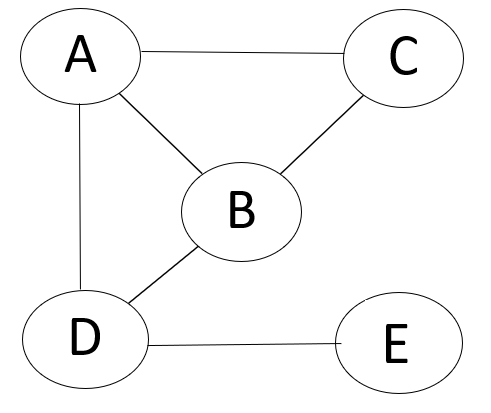
\includegraphics[width=0.5\textwidth, center]{graph}
    
    The adjacency matrix A of the above graph will be as shown below:
    % INSERT MATRIX A
    \begin{equation*}
    \begin{bmatrix}
    - & 1 & 1 & 1 & 0 \\
    1 & - & 1 & 1 & 0 \\
    1 & 1 & - & 0 & 0 \\
    1 & 1 & 0 & - & 1 \\
    0 & 0 & 0 & 1 & - \\

    \end{bmatrix}
    \end{equation*}
    
    Let’s assume that in the above graph, the importance of each node is measured by its degree, such that the higher the degree of a node, the more important it is in the graph. Degrees of various nodes are shown below:
    % INSERT TABLE

    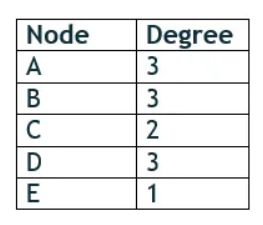
\includegraphics[center]{Table}
    
    % \begin{table}
    % \centering
    % \begin{tabular}{|c|c|}
    % \hline
    % Node & Degree \\
    % \hline
    % A & 3 \\
    % B & 3 \\
    % C & 2 \\ 
    % D & 3 \\
    % E & 1 \\
    % \hline
    % \end{tabular}
    % \end{table}
    
    The above can also be represented as a vector V as shown below:
    % INSERT VECTOR

    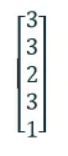
\includegraphics[center]{Vector}

    Mathematically the Eigen Vector Centrality is calculated as below:
    % INSERT MULTIPLICATION 

    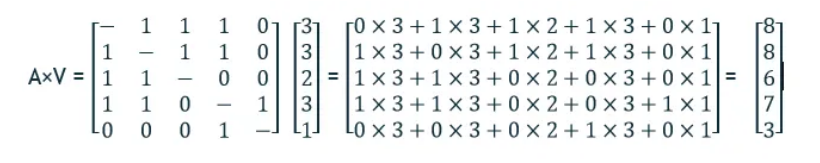
\includegraphics[width=0.9\textwidth,center]{Multiplication}

    The resultant 1-D vector in the above equation gives the Eigen Vector Centrality (EVC) score for each of the nodes in the graph.

    The effect of the first iteration of multiplication can be visualized as shown below:
    % INSERT TRANSFORM

    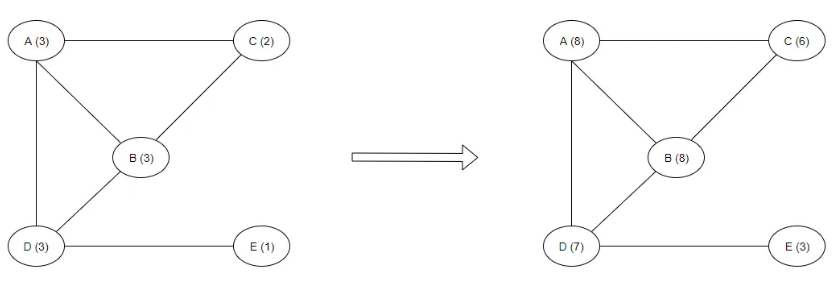
\includegraphics[width=0.9\textwidth,center]{Transform}

    As you can see above, nodes A and B both have a high score of 8 since both of them are connected to multiple nodes with high degrees (importance) while node E has a score of 3 since it is only connected to a single node of degree 3.
    
    Observe that the EVC score value for each node in the resultant vector is nothing but the sum of degrees of its neighbouring nodes.
    
    Multiplying the resultant vector again with the adjacency matrix of the graph helps the EVC score spread out in the graph to get a more globally prominent EVC score vs a localized EVC score for each node in the graph. After the first iteration of multiplication, each node’s EVC score is a function of only its direct (first degree) neighbours, thus is a localized score which might not be accurate at a global level in the graph.

    Thus, the following observations can be made:
    
    (I)     After the first iteration of multiplication, each node gets its EVC score from its direct(first degree) neighbours.
    
    (II)	In the second iteration, when we multiply the resultant vector again with the adjacency matrix, each node again gets its EVC score from its direct neighbours but the difference in the second iteration is that this time, the scores of the direct neighbours have already been impacted by their own direct(1st degree) neighbours previously(from the first iteration of multiplication) which eventually helps the EVC score of any node to be a function of its 2nd degree neighbouring nodes as well.
    
    (III)	In subsequent iterations of multiplication, the EVC score of graph nodes keeps getting updated by getting impacted by EVC scores from neighbouring nodes of farther degrees (3rd, 4th and so on).

    Repeated multiplication makes the EVC score of every node eventually be a function of or dependent on several degrees of its neighbouring nodes, thereby providing a globally accurate EVC score for each node. Usually, the process of multiplying the EVC vector with the adjacency matrix is repeated until the EVC values for nodes in the graph reach an equilibrium or stop showing the appreciable change.

    One sample application of EVC is the calculation of Page Rank or Page Rank algorithm used by Google and many other companies to rank web pages on the internet by relevance. Page Rank is a direct variant of EVC. Web pages on the World Wide Web have links that point to/from other web pages. You can think of each web page as a node in the graph and each outgoing/incoming link as a directed edge leading to/from another web page on the web, thereby making up the whole World Wide Web graph. The graph of web pages in the world wide web undergoes several iterations of EVS calculation so as to calculate globally accurate relevance rankings of each web page. The web pages with high EVC scores can then be targeted for marketing and other commercial purposes.
    
\end{itemize}

\end{document}